\begin{figure}[t]
\centering
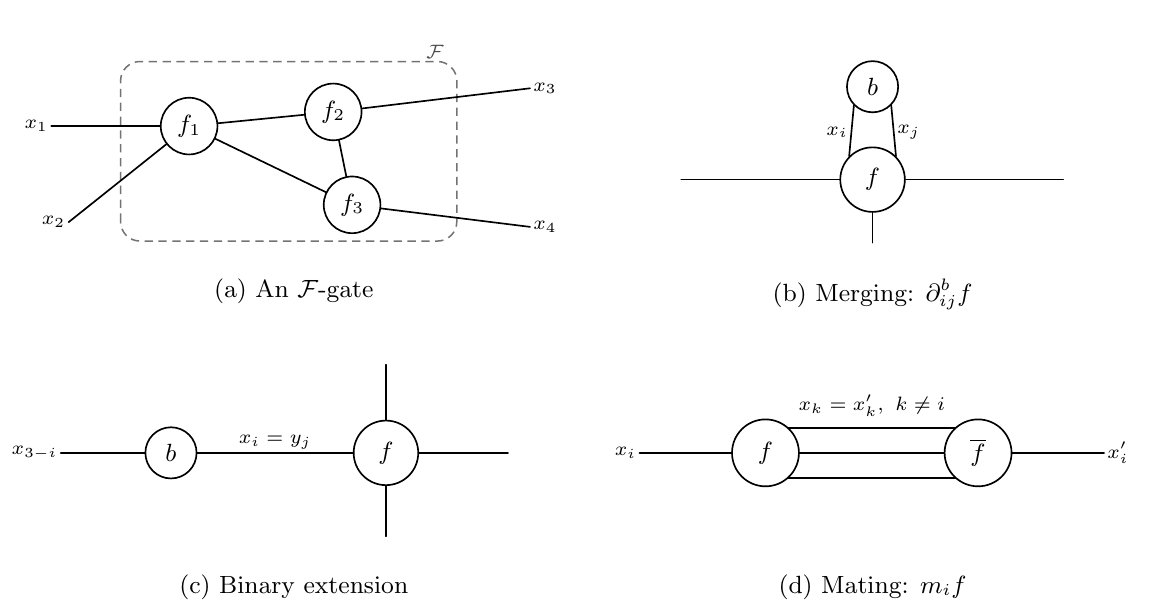
\begin{tikzpicture}[
    wire/.style={draw=black, line width=0.6pt, line cap=round},
    boundary/.style={draw=black!55, densely dashed, line width=0.55pt,
        rounded corners=7pt},
    signature/.style={draw=black, circle, fill=white, minimum size=7.2mm,
        inner sep=0pt, line width=0.6pt, font=\small},
    small signature/.style={signature, minimum size=6.5mm},
    port label/.style={font=\scriptsize, inner sep=1pt},
    panel label/.style={font=\small, anchor=north}
]

% (a) An F-gate
\begin{scope}[shift={(0,3.75)}]
    \path[use as bounding box] (0,0) rectangle (6.75,3.35);

    \draw[boundary] (1.18,0.64) rectangle (5.45,2.92);
    \node[port label, anchor=south east, text=black!70]
        at (5.33,2.92) {$\mathcal F$};

    \draw[wire] (0.30,2.10) -- (2.05,2.10);
    \draw[wire] (0.52,0.88) -- (2.05,2.10);
    \draw[wire] (2.05,2.10) -- (3.88,2.28);
    \draw[wire] (2.05,2.10) -- (4.12,1.10);
    \draw[wire] (3.88,2.28) -- (4.12,1.10);
    \draw[wire] (3.88,2.28) -- (6.38,2.58);
    \draw[wire] (4.12,1.10) -- (6.38,0.82);

    \node[signature] at (2.05,2.10) {$f_1$};
    \node[signature] at (3.88,2.28) {$f_2$};
    \node[signature] at (4.12,1.10) {$f_3$};

    \node[port label, left] at (0.30,2.10) {$x_1$};
    \node[port label, left] at (0.52,0.88) {$x_2$};
    \node[port label, right] at (6.38,2.58) {$x_3$};
    \node[port label, right] at (6.38,0.82) {$x_4$};
    \node[panel label] at (3.38,0.28)
        {\textup{(a)} An $\mathcal F$-gate};
\end{scope}

% (b) Merging two variables of f using b
\begin{scope}[shift={(7.35,3.75)}]
    \path[use as bounding box] (0,0) rectangle (6.75,3.35);

    \node[small signature] (merge-b) at (3.38,2.60) {$b$};
    \node[signature, minimum size=8.2mm] (merge-f) at (3.38,1.42) {$f$};

    \draw[wire] (merge-b.225) --
        node[port label, left, pos=0.53] {$x_i$} (merge-f.135);
    \draw[wire] (merge-b.315) --
        node[port label, right, pos=0.53] {$x_j$} (merge-f.45);
    \draw[wire] (0.95,1.42) -- (merge-f.180);
    \draw[wire] (merge-f.0) -- (5.80,1.42);
    \draw[wire] (3.38,0.62) -- (merge-f.270);

    \node[panel label] at (3.38,0.28)
        {\textup{(b)} Merging: $\partial_{ij}^{b}f$};
\end{scope}

% (c) Binary extension
\begin{scope}
    \path[use as bounding box] (0,0) rectangle (6.75,3.35);

    \node[small signature] (ext-b) at (1.82,1.70) {$b$};
    \node[signature, minimum size=8.2mm] (ext-f) at (4.55,1.70) {$f$};

    \draw[wire] (0.42,1.70) -- (ext-b.180);
    \draw[wire] (ext-b.0) --
        node[port label, above] {$x_i=y_j$} (ext-f.180);
    \draw[wire] (ext-f.0) -- (6.10,1.70);
    \draw[wire] (4.55,2.82) -- (ext-f.90);
    \draw[wire] (4.55,0.64) -- (ext-f.270);

    \node[port label, left] at (0.42,1.70) {$x_{3-i}$};
    \node[panel label] at (3.38,0.28)
        {\textup{(c)} Binary extension};
\end{scope}

% (d) Mating f with its conjugate
\begin{scope}[shift={(7.35,0)}]
    \path[use as bounding box] (0,0) rectangle (6.75,3.35);

    \draw[wire] (0.42,1.70) -- (2.02,1.70);
    \draw[wire] (2.02,2.02) -- (4.72,2.02);
    \draw[wire] (2.02,1.70) -- (4.72,1.70);
    \draw[wire] (2.02,1.38) -- (4.72,1.38);
    \draw[wire] (4.72,1.70) -- (6.32,1.70);

    \node[signature, minimum size=8.5mm] at (2.02,1.70) {$f$};
    \node[signature, minimum size=8.5mm] at (4.72,1.70) {$\overline f$};

    \node[port label, left] at (0.42,1.70) {$x_i$};
    \node[port label, right] at (6.32,1.70) {$x_i'$};
    \node[port label, fill=white] at (3.37,2.30)
        {$x_k=x_k',\ k\ne i$};
    \node[panel label] at (3.38,0.28)
        {\textup{(d)} Mating: $\mathfrak m_i f$};
\end{scope}

\end{tikzpicture}
\caption{Basic gadget constructions.
\textup{(a)} An $\mathcal F$-gate, with every internal signature in
$\mathcal F$.
\textup{(b)} Merging the variables $x_i$ and $x_j$ of $f$ with the binary
signature $b$, producing $\partial_{ij}^{b}f$.
\textup{(c)} A binary extension formed by identifying $x_i$ of $b$ with
$y_j$ of $f$.
\textup{(d)} Mating $f$ with $\overline f$ on all variables except $x_i$,
producing $\mathfrak m_i f$; the three parallel wires represent these
$n-1$ contractions.
Joined half-edges are contracted, whereas unjoined half-edges are free
variables.}
\label{fig:gadget-constructions}
\end{figure}
